\chapter{Methods}
The experiment required a Stirling engine, a Fresnel lens, Arduino UNO microcontroller, DC motor, thermocouple, and other circuitry as listed in each section below.

\begin{figure}[ht]
    \centering
    \includegraphics[width=\textwidth]{diagrams/complete}
    \caption[Experimental setup]{Figure of setup. (a) Stirling engine (b) brushless DC motor (c) microSD breakout board (d) LCD screen (e) 8-bit shift register (f) thermocouple module (g) Arduino UNO}
    \label{fig:setup}
\end{figure}

\section{Stirling Engine}

    While the experiment originally called for the development of a Stirling engine, one was not completed in time. Alternatively, the purchase of a Stirling engine by Sunnytech allowed for more immediate data collection. In the original design, Borosilicate glass syringes were used as pistons because they can be used at high temperatures and the plunger makes an air-tight seal. The rest of the engine was machined out of aluminum, with some small parts such as the flywheels and gears made from plastic. Due to time constraints, this engine has yet to run.
    
    \begin{figure}[H]
        \centering
        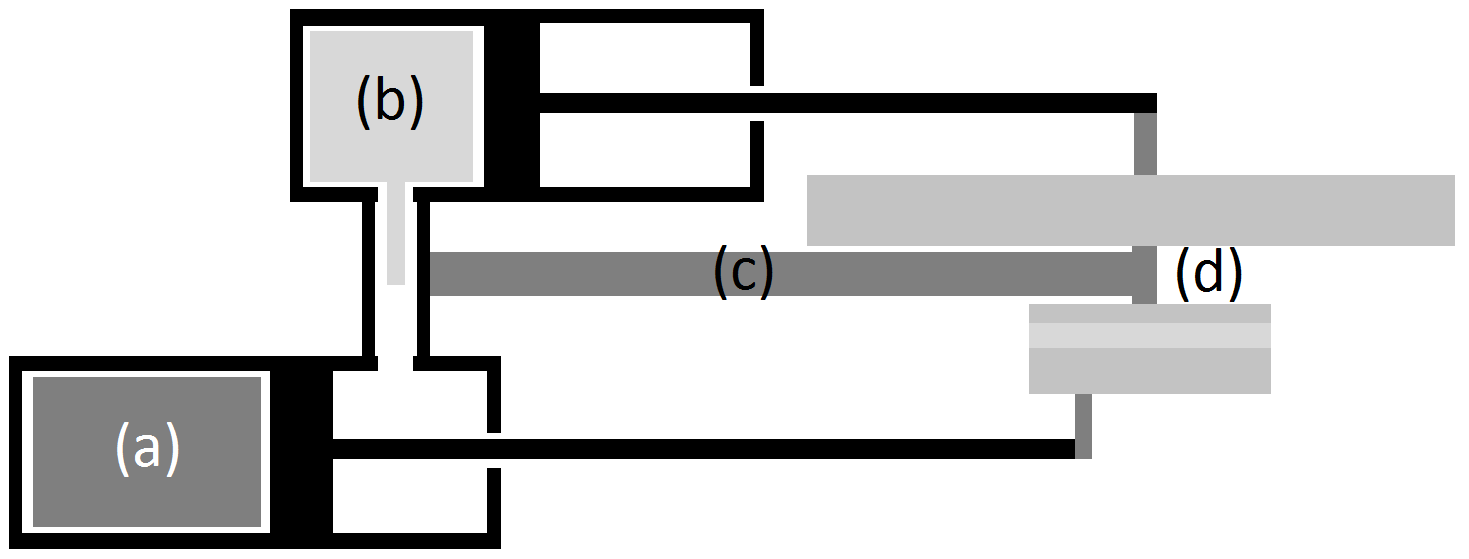
\includegraphics[width=\textwidth]{diagrams/stirling2}
        \caption[Stirling engine]{Simplified diagram of the Stirling engine used. Notice the oscillatory alignment of the pistons is such that they have a phase difference of \(\frac{\pi}{2}\). (a) Hot piston (b) cold piston (c) brace to hold engine together (d) flywheels.}
        \label{fig:stirling}
    \end{figure}

\section{Solar Collector}

    An 8.3" by 11.75" Fresnel lens was used as the solar energy collector. The flat design of a Fresnel lens allowed for easy modification of the amount of light to be passed through the lens.  As seen in Figure \ref{fig:fresnel}, slides of varying hole size were placed over the lens such that the area could be measured. The focal point of the solar collector setup was then positioned on the hot cylinder of the Stirling engine.
    
    \begin{figure}[H]
        \centering
        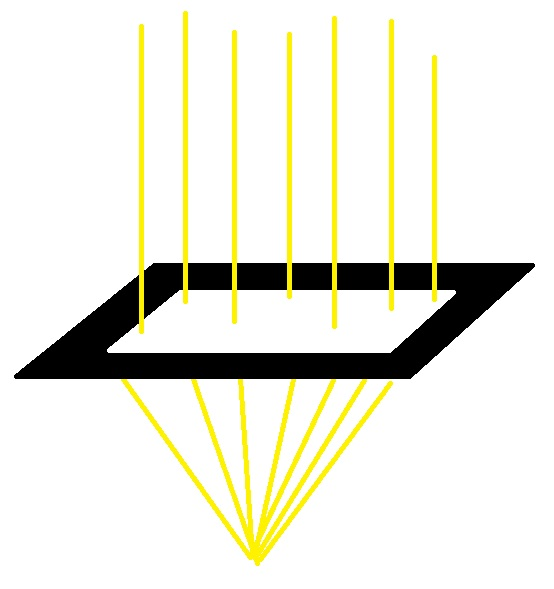
\includegraphics[width=0.3\textwidth]{diagrams/fresnel}
        \caption[Fresnel lens]{As light passes through the plane of the Fresnel lens, it converges to a focal point. The thick rectangle represents the apertures which were laid over the lens to modify the amount of light which passes through the lens.}
        \label{fig:fresnel}
    \end{figure}

\section{Arduino Data Collection}

    An Arduino UNO microcontroller board was used for data collection due to its ability to read and write information and has many inputs and outputs. A K-type thermocouple with the Arduino MAX6675 module were used to read temperature data from the hot piston of the Stirling engine and send the information to the Arduino. A small brushless direct current (D.C.) motor taken from a computer fan was was attached to the flywheel of the engine and ran in 'reverse' as a generator in order to produce a voltage. Since the brushless D.C. motor produces an alternating current (A.C.) when running in reverse, this voltage was passed through a full-wave rectifier to convert the A.C. to D.C. for easier data analysis. This voltage was used as the output from the system which was recorded. This then was read by an analog input pin of the Arduino. An Adafruit ADA254 MicroSD card breakout board was used to record data. The Arduino also output data to the IC74HC59N 8-bit shift register to run the LCM1602C LCD screen for a live data feed. These parts can be seen labeled in Figure \ref{fig:circuit}.
    
    \begin{figure}[H]
        \centering
        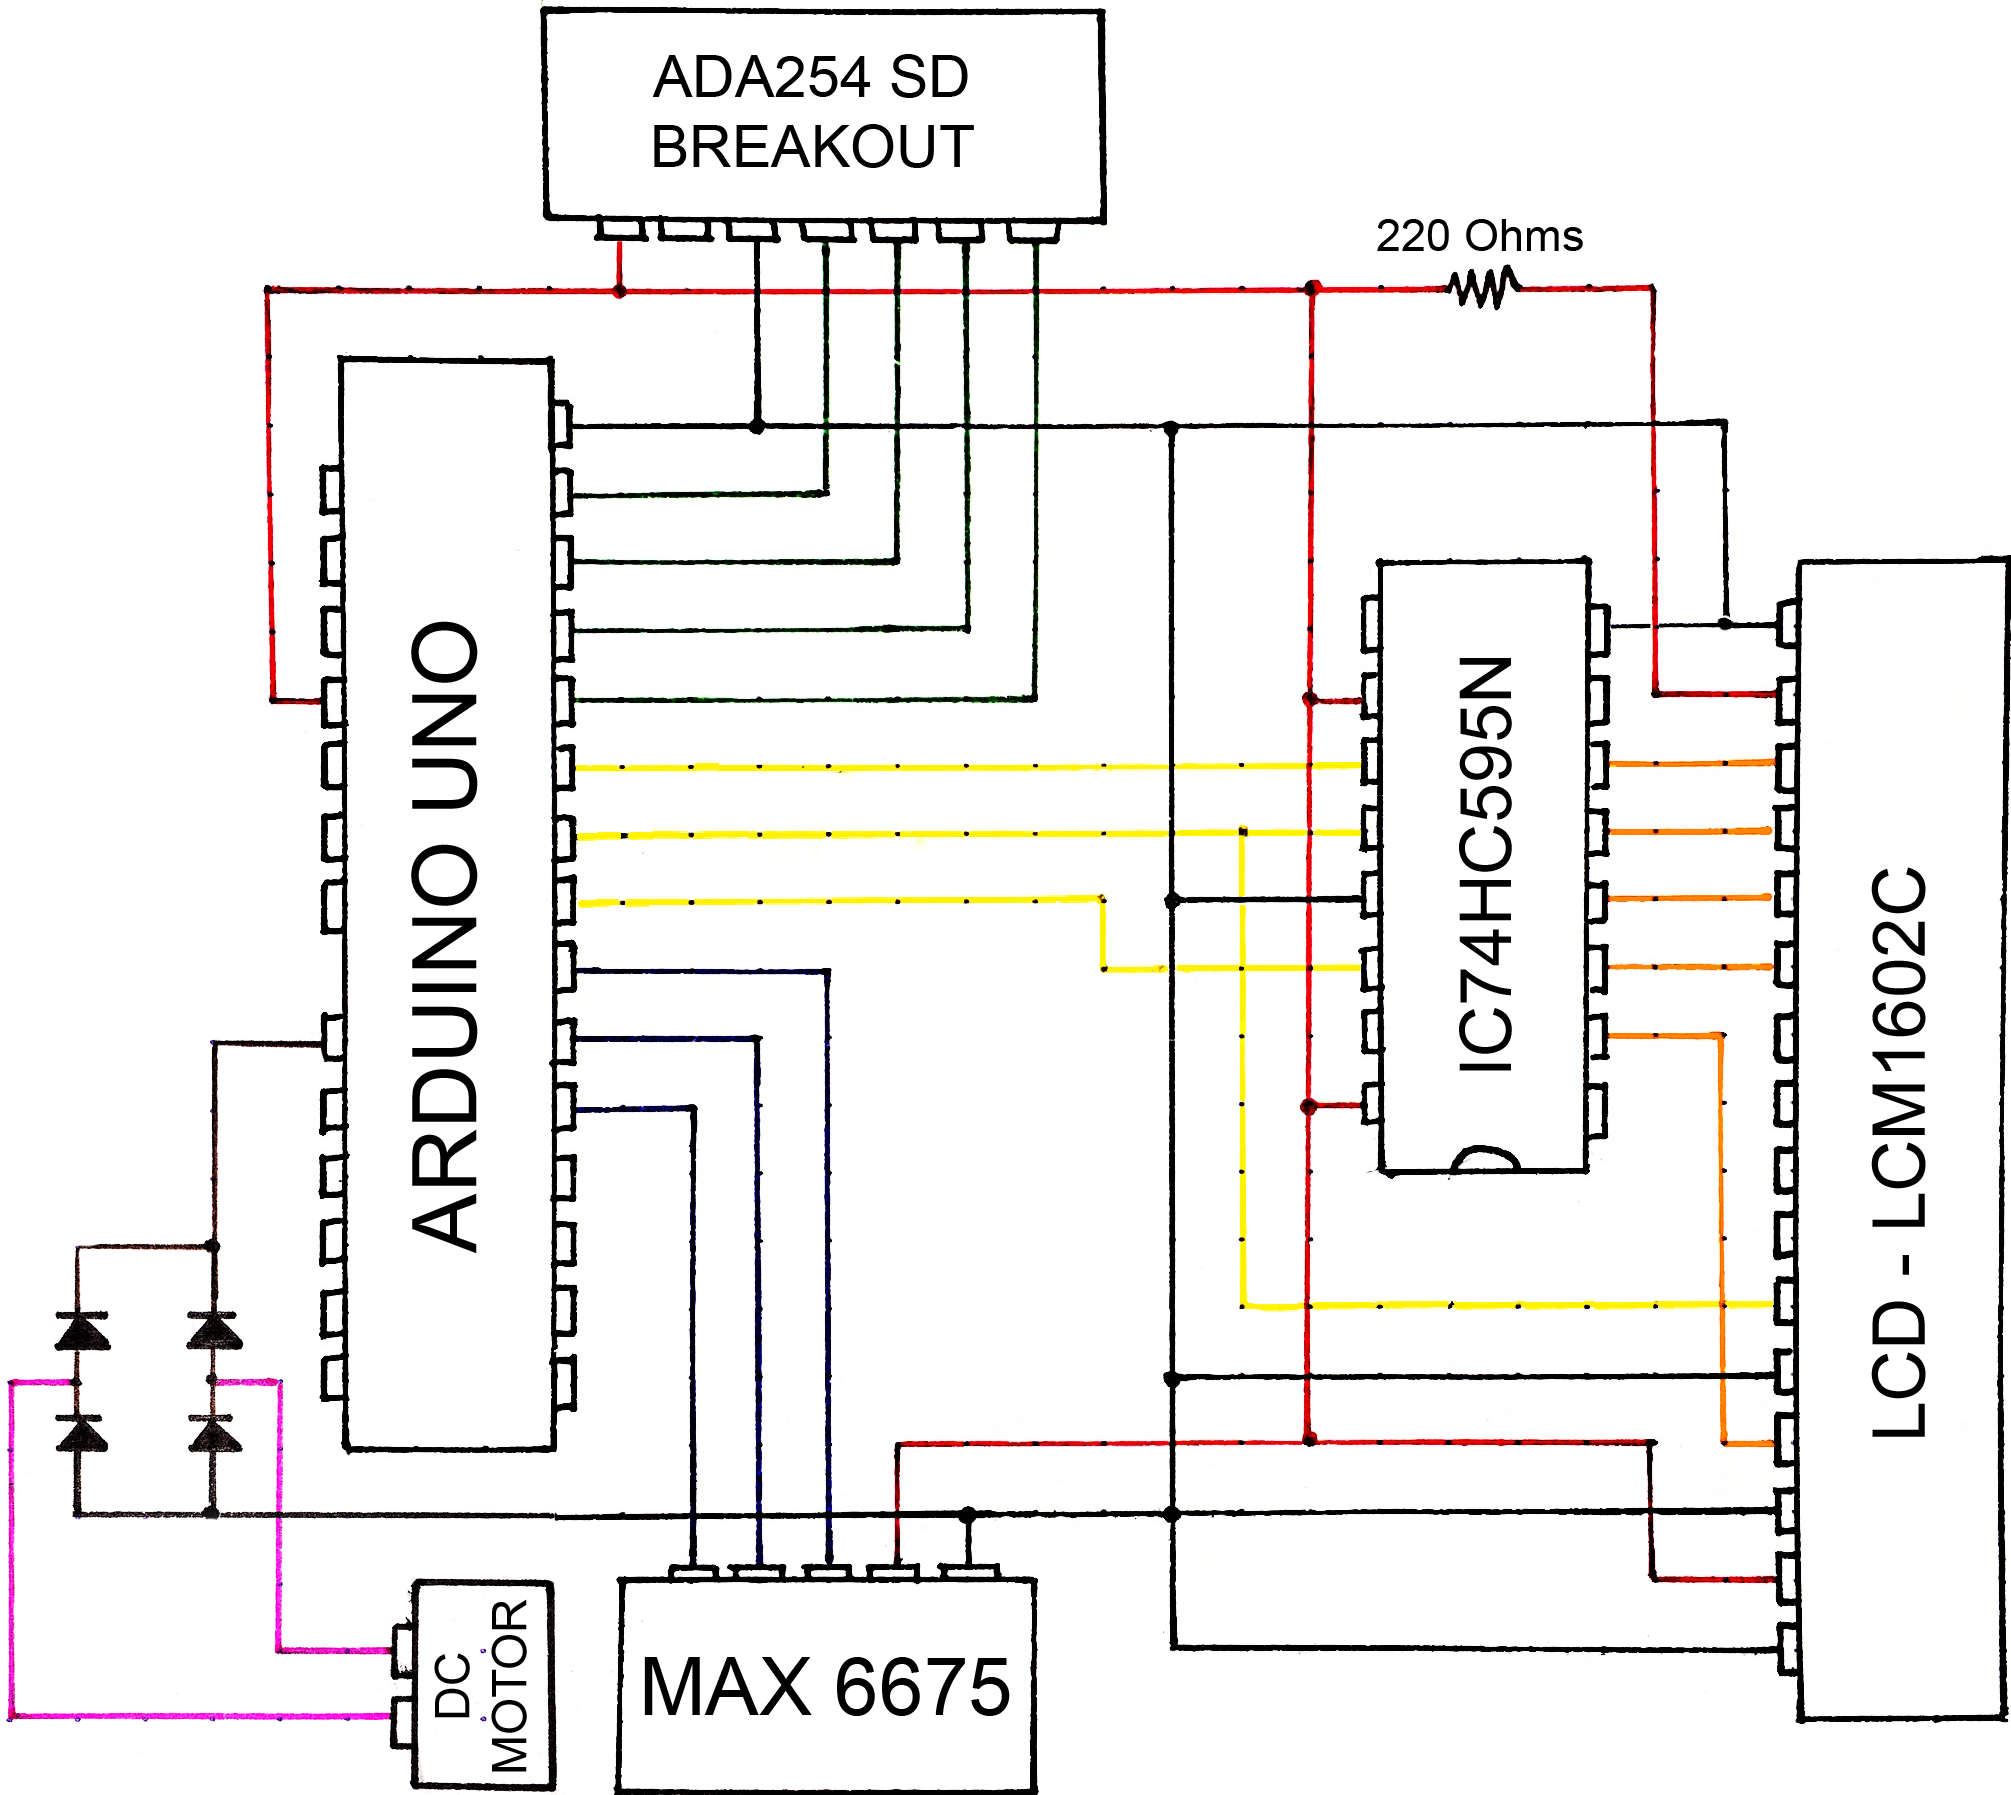
\includegraphics[width=\textwidth]{diagrams/circuit}
        \caption[Circuit diagram]{Circuit diagram of electrical components.}
        \label{fig:circuit}
    \end{figure}